% comment out for student version
\ifdefined\Student\relax\else\def\Teacher{}\fi

\documentclass[12pt]{article}

\title{Recursive Methods}
\author{Chris Mayfield, Dee Weikle, and Helen Hu}
\date{Summer 2021}

%\ProvidesPackage{cspogil}

% fonts
\usepackage[utf8]{inputenc}
\usepackage[T1]{fontenc}
\usepackage{mathpazo}

% spacing
\usepackage[margin=2cm]{geometry}
\renewcommand{\arraystretch}{1.4}
\setlength{\parindent}{0pt}

% orphans and widows
\clubpenalty=10000
\widowpenalty=10000
\pagestyle{empty}

% figures and tables
\usepackage{graphicx}
\usepackage{multicol}
\usepackage{tabularx}
\usepackage{wrapfig}

% fixed-width columns
\usepackage{array}
\newcolumntype{L}[1]{>{\raggedright\let\newline\\\arraybackslash\hspace{0pt}}m{#1}}
\newcolumntype{C}[1]{>{\centering\let\newline\\\arraybackslash\hspace{0pt}}m{#1}}
\newcolumntype{R}[1]{>{\raggedleft\let\newline\\\arraybackslash\hspace{0pt}}m{#1}}

% include paths
\makeatletter
\def\input@path{{Models/}{../../Models/}}
\graphicspath{{Models/}{../../Models/}}
\makeatother

% colors
\usepackage[svgnames,table]{xcolor}
\definecolor{bgcolor}{HTML}{FAFAFA}
\definecolor{comment}{HTML}{007C00}
\definecolor{keyword}{HTML}{0000FF}
\definecolor{strings}{HTML}{B20000}

% table headers
\newcommand{\tr}{\bf\cellcolor{Yellow!10}}

% syntax highlighting
\usepackage{textcomp}
\usepackage{listings}
\lstset{
    basicstyle=\ttfamily\color{black},
    backgroundcolor=\color{bgcolor},
    numberstyle=\scriptsize\color{comment},
    commentstyle=\color{comment},
    keywordstyle=\color{keyword},
    stringstyle=\color{strings},
    columns=fullflexible,
    keepspaces=true,
    showlines=true,
    showstringspaces=false,
    upquote=true
}

% code environments
\newcommand{\java}[1]{\lstinline[language=java]{#1}}%[
\lstnewenvironment{javalst}{\lstset{language=java,backgroundcolor=}}{}
\lstnewenvironment{javabox}{\lstset{language=java,frame=single,numbers=left}\quote}{\endquote}

% PDF properties
\usepackage[pdftex]{hyperref}
\urlstyle{same}
\makeatletter
\hypersetup{
  pdftitle={\@title},
  pdfauthor={\@author},
  pdfsubject={\@date},
  pdfkeywords={},
  bookmarksopen=false,
  colorlinks=true,
  citecolor=black,
  filecolor=black,
  linkcolor=black,
  urlcolor=blue
}
\makeatother

% titles
\makeatletter
\renewcommand{\maketitle}{\begin{center}\LARGE\@title\end{center}}
\makeatother

% boxes [optional height]
\newcommand{\emptybox}[1][10em]{
\vspace{1em}
\begin{tabularx}{\linewidth}{|X|}
\hline\\[#1]\hline
\end{tabularx}}

% models
\newcommand{\model}[1]{\section{#1}\nopagebreak}
\renewcommand{\thesection}{Model~\arabic{section}}

% questions
\newcommand{\quest}[1]{\subsection*{Questions~ (#1)}}
\newcounter{question}
\newcommand{\Q}{\vspace{1em}\refstepcounter{question}\arabic{question}.~ }
\renewcommand{\thequestion}{\#\arabic{question}}

% sub-question lists
\usepackage{enumitem}
\setenumerate[1]{label=\alph*)}
\setlist{itemsep=1em,after=\vspace{1ex}}

% inline answers
\definecolor{answers}{HTML}{C0C0C0}
\newcommand{\ans}[1]{%
\ifdefined\Student
    \leavevmode\phantom{~~\textcolor{answers}{#1}}
\else
    ~~\textcolor{answers}{#1}
\fi}

% longer answers [optional height]
\newsavebox{\ansbox}
\newenvironment{answer}[1][4em]{
\nopagebreak
\begin{lrbox}{\ansbox}
\begin{minipage}[t][#1]{\linewidth}
\color{answers}
}{
\end{minipage}
\end{lrbox}
\ifdefined\Student
    \phantom{\usebox{\ansbox}}%
\else
    \usebox{\ansbox}%
\fi}


\begin{document}

\maketitle

Sometimes when solving a problem, we can compute the solution of a simpler version of the {\it same problem}.
Eventually we reach the most basic version, for which the answer is trivial.

\rolenames

\guide{
  \item Identify the base case and recursive step of the factorial method.
  \item Trace a recursive method by hand and predict its final output.
  \item Explain what happens in memory when a method calls itself.
}{
  \item Evaluating mathematical sequences to gain insight on recursion. (Information Processing)
}{
This activity is a first introduction to recursion using two mathematical examples: factorial and summation.
Students learn how to read and trace recursive methods, not how to formulate recursive solutions to problems.
Let students wrestle with these difficult concepts, and don't give too much help on individual questions.

Keep an eye on questions 1--3, and if a team is getting off track, have them compare answers with a neighboring team.
You may need to point out that $!$ in mathematics means \emph{factorial}, but \java{!} in Java means \emph{not}.
It's unfortunately common that operators have slightly different meanings in different languages.

Report out on \ref{factjava} and \ref{output} by having teams write their answers on the board.
Ideally there will be slightly different (incorrect) answers, which will lead to a discussion.
Paste \textit{Recursion.java} into \href{https://cscircles.cemc.uwaterloo.ca/java_visualize/}{Java Visualizer} and step through the code as a live demo.
After \ref{stackover}, introduce the term \emph{stack overflow} and make the connection to the \emph{call stack} visualization in Java Visualizer.

Depending on how long you report out, \ref{factorial.tex} could take an additional 5--10 minutes.
\ref{summation.tex} should move a bit faster, since summation is almost identical to factorial.
Invite presenters to write their team's solution to \ref{diagram} on the board.
Address any misconceptions about variables, parameter passing, and return values.

Key questions: \ref{key1}, \ref{stackover}, \ref{diagram}

Source files: \src{Act08}{Recursion.java}
}

\model{Factorial Function}

''In mathematics, the factorial of a non-negative integer $n$, denoted by $n!$, is the product of all positive integers less than or equal to $n$. For example, $5! = 5 \times 4 \times 3 \times 2 \times 1 = 120$.''

\smallskip\hfill
Source: \url{https://en.wikipedia.org/wiki/Factorial}

\begin{center}
\begin{tabular}{|C{1cm}|C{1cm}|}
\hline
\tr n & \tr n! \\
\hline
1 & 1 \\
\hline
2 & 2 \\
\hline
3 & 6 \\
\hline
4 & 24 \\
\hline
5 & 120 \\
\hline
6 & 720 \\
\hline
\end{tabular}
\end{center}


\quest{15 min}


\Q \label{fact4} Consider two different ways to show how to calculate 4!

\begin{enumerate}
\item Write out all numbers that need to be multiplied

4! = \ans{4 * 3 * 2 * 1}

\item Rewrite the expression using 3!

4! = \ans{4 * 3!}
\end{enumerate}


\Q Write an expression similar to \ref{fact4}b showing how each factorial can be calculated in terms of a simpler factorial.

\begin{enumerate}
\item 3! = \ans{3 * 2!}
\item 2! = \ans{2 * 1!}
\item 100! = \ans{100 * 99!}
\item $n!$ = \ans{$n * (n - 1)!$}
\end{enumerate}


\Q What is the value of 1! based on the model? Does it make sense to define 1! in terms of a simpler factorial?

\newpage
\model{Summation}
% based on Model 2 of Activity 12 - Recursion by Helen Hu, with modifications by Dee Weikle

''In mathematics, \emph{summation} (capital Greek sigma symbol: $\Sigma$) is the addition of a sequence of numbers; the result is their sum or total.''

$$ \sum_{i=1}^{100} i = 1 + 2 + 3 + \ldots + 100 = 5050 $$

\smallskip\hfill
Source: \url{https://en.wikipedia.org/wiki/Summation}


\quest{20 min}


\Q \label{sum4}
Consider how to calculate $\sum\limits_{i=1}^{4} i = 10$.

\begin{enumerate}
\item Write out all the numbers that need to be added:

$\sum\limits_{i=1}^{4} i =$ \ans{4 + 3 + 2 + 1}

\item Show how this sum can be calculated in terms of a smaller summation.

$\sum\limits_{i=1}^{4} i =$ \ans{4 + $\sum\limits_{i=1}^{3} i$}
\end{enumerate}


\Q Write an expression similar to \ref{sum4}b showing how any summation of $n$ integers can be calculated in terms of a smaller summation.

\begin{center}
$\sum\limits_{i=1}^{n} i =$ \ans{n + $\sum\limits_{i=1}^{n-1} i$}
\end{center}


\Q What is the base case of the summation? (Write the complete formula, not just the value.)

\begin{answer}
$$\sum\limits_{i=1}^{1} i = 1$$
\end{answer}


\Q Implement a recursive method \java{summation} that takes a single parameter \java{n} and returns the sum $1 + 2 + \ldots + n$.
It should only have an \java{if} statement and two \java{return} statements.

\vspace{-1ex}
\begin{answer}[10em]
\begin{javaans}
public static int summation(int n) {
    if (n == 1) {
        return 1;
    } else {
        return n + summation(n - 1);
    }
}
\end{javaans}
\end{answer}


\Q Discuss how the \java{factorial} method below uses temporary variables.
What lines would you have to change to implement the \java{summation} method instead?

\begin{multicols}{2}

\vspace{1ex}
\begin{javalst}
public static int factorial(int n) {
    if (n == 0) {
        return 1;  // base case
    }
    int recurse = factorial(n - 1);
    int result = n * recurse;
    return result;
}
\end{javalst}

\columnbreak

\begin{answer}[5em]
First rename the method to \java{summation}.
Then change the base case to be \texttt{if (n == 1)}.
The recursive step must invoke \java{summation}, and the result must add terms instead of multiply.
\end{answer}

\end{multicols}


\Q \label{diagram}
Here is a stack diagram of ~\java{factorial(3)} when invoked from \java{main}.
Draw a similar diagram for \java{summation(3)} as described in the previous question.

\vspace{1em}
\begin{minipage}{0.48\linewidth}

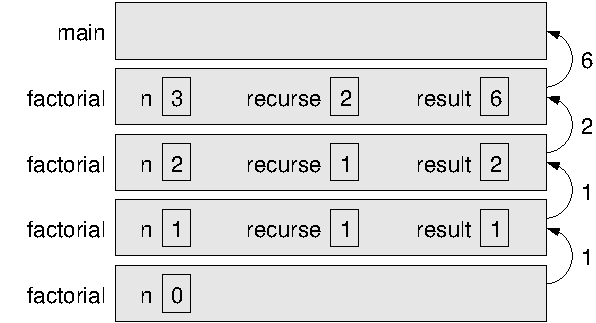
\includegraphics[width=\linewidth]{stack3.pdf}

\end{minipage}
\hfill
\begin{minipage}{0.48\linewidth}

\begin{answer}[115pt]
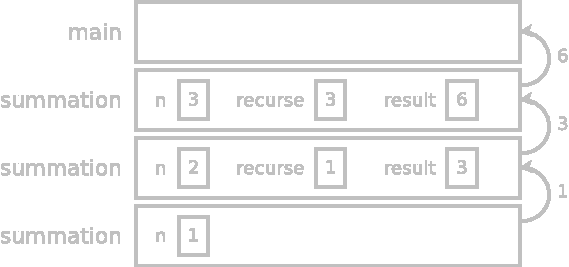
\includegraphics[width=\linewidth]{stack3-ans.pdf}
\end{answer}

\end{minipage}
\vspace{1em}


\Q Why are there no values for \java{recurse} and \java{result} in the stack diagram for the last call to \java{factorial} (when \java{n == 0})?

\begin{answer}
The method returns without declaring and using those variables.
\end{answer}


\Q Looking at the stack diagram, how is it possible that the parameter \java{n} can have multiple values in memory at the same time?

\begin{answer}
Each distinct method call has its own memory for parameters and local variables.
The value of \java{n - 1} in the first method call becomes the value of \java{n} in the next.
\end{answer}


\end{document}
